\chapter{Study of the parameters of the fit}
    \label{app:FitResults}

This appendix collects further details on the fit performed in the analysis shown in Chapter~\ref{chapter:MonojetAnalysis}, which allows to estimate the normalization factors and the systematic uncertainties of the different background processes.

The correlation between the parameters of the fit for the signal selection M1 is shown in Figure~\ref{fig:corrMatrix}.
The three normalization factors used in the analysis (\texttt{mu\_Ele}, \texttt{mu\_Wmn} and \texttt{mu\_Zmm}) are highly correlated among themselves, as a consequence of the cross contamination between the background processes in the different control regions.
Correlation between the normalization factors and some systematic sources are also significant, for example in the case of the \texttt{alpha\_ktfac} or the \texttt{alpha\_qfac} nuisance parameters, for which their systematic effects are compensated by the normalization factors, computed in the control regions.
Finally, nuisance parameters for the systematic uncertainties are practically uncorrelated among themselves.
The fit parameters in the other signal selections show similar correlation patterns.

\begin{figure}[!ht]
  \begin{center}
    \mbox{
      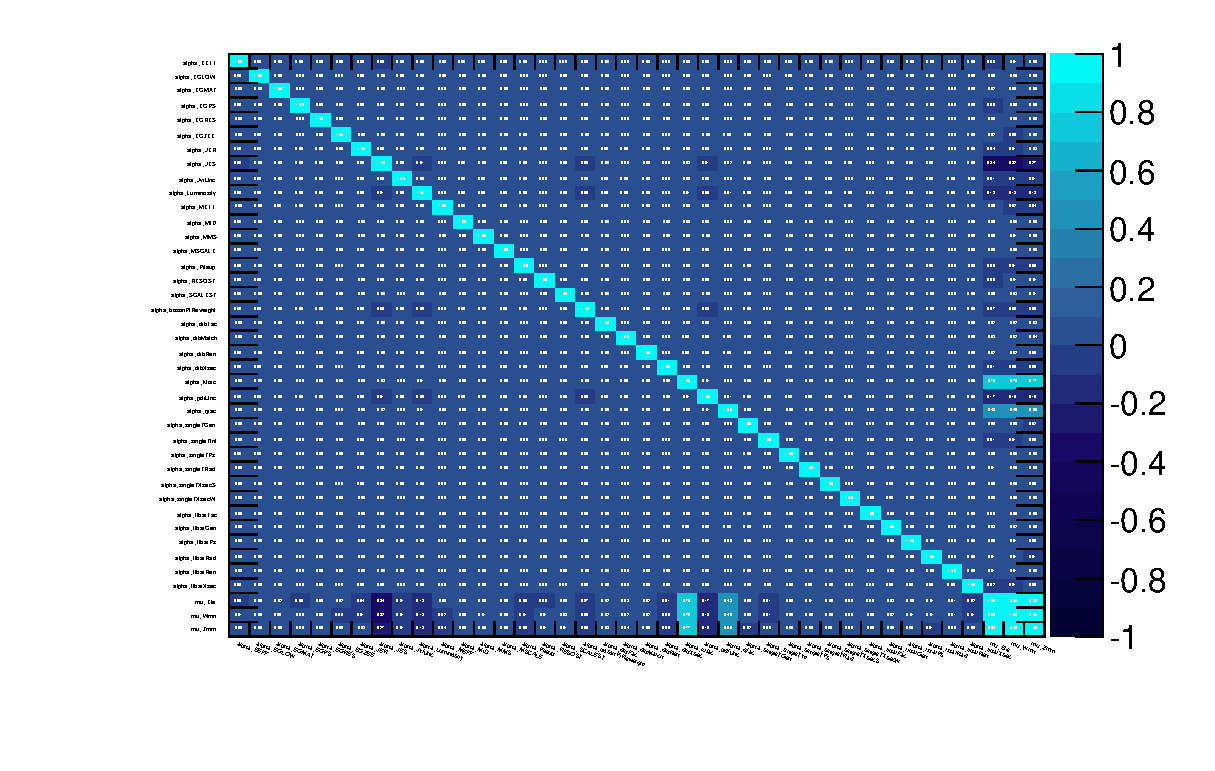
\includegraphics[width=0.995\textwidth]{MonojetAnalysis/Figures/corrMatrix_Stop_M1.eps}
    }
  \end{center}
  \caption[Correlations among the different nuisance parameters and normalization factors after performing the fits with the background-only setup in the M1 signal selection.]{Correlations among the different nuisance parameters and normalization factors after performing the fits with the background-only setup in the M1 signal selection.}
  \label{fig:corrMatrix}
\end{figure}

The nuisance parameters for the selection M1 are shown in Table~\ref{tab:fitparameters_Stop_M1}.
After the fit, all of them lay below $0.001$.
The fact that these parameters have changed by less than $0.1\%$ with respect to the value to which they were initialized is an indication that there is no need for a significant profile of the systematic uncertainties to accommodate the data.
The central values of the nuisance parameters for all selections are shown in Figures~\ref{fig:corrMatrix_M1M2M3} and \ref{fig:corrMatrix_M4M5M6}.

%--- \ref{tab:fitparameters_Stop_M1}

\begin{table}
\begin{center}
\setlength{\tabcolsep}{0.0pc}
\begin{tabular*}{\textwidth}{@{\extracolsep{\fill}}lcc}
\noalign{\smallskip}\hline\noalign{\smallskip}
Parameter                                   &    initial value and error & fitted value and error       \\
\noalign{\smallskip}\hline\noalign{\smallskip}
%%
alpha\_JvfUnc & $0.00\pm 1.00$  & $ \phantom{-}0.0000\pm 0.9893$  \\
%%
alpha\_MEFF & $0.00\pm 1.00$  & $ \phantom{-}0.0001\pm 0.9932$  \\
%%
alpha\_JES & $0.00\pm 1.00$  & $ \phantom{-}0.0014\pm 0.9769$  \\
%%
alpha\_MMS & $0.00\pm 1.00$  & $ -0.0000\pm 0.9905$  \\
%%
alpha\_RESOST & $0.00\pm 1.00$  & $ \phantom{-}0.0000\pm 0.9933$  \\
%%
alpha\_MSCALE & $0.00\pm 1.00$  & $ \phantom{-}0.0000\pm 0.9934$  \\
%%
alpha\_JER & $0.00\pm 1.00$  & $ \phantom{-}0.0000\pm 0.9931$  \\
%%
alpha\_pdfUnc & $0.00\pm 1.00$  & $ \phantom{-}0.0012\pm 0.9864$  \\
%%
alpha\_bosonPtReweight & $0.00\pm 1.00$  & $ \phantom{-}0.0002\pm 0.9928$  \\
%%
alpha\_singleTGen & $0.00\pm 1.00$  & $ -0.0000\pm 0.9932$  \\
%%
alpha\_Pileup & $0.00\pm 1.00$  & $ \phantom{-}0.0000\pm 0.9932$  \\
%%
alpha\_MID & $0.00\pm 1.00$  & $ -0.0000\pm 0.9935$  \\
%%
alpha\_dibRen & $0.00\pm 1.00$  & $ -0.0000\pm 0.9919$  \\
%%
alpha\_EGRES & $0.00\pm 1.00$  & $ -0.0000\pm 0.9929$  \\
%%
alpha\_singleTXsecS & $0.00\pm 1.00$  & $ -0.0001\pm 0.9933$  \\
%%
alpha\_qcdNorm & $0.00\pm 1.00$  & $ \phantom{-}0.0000\pm 1.0000$  \\
%%
alpha\_EEFF & $0.00\pm 1.00$  & $ \phantom{-}0.0000\pm 0.9931$  \\
%%
alpha\_ttbarRad & $0.00\pm 1.00$  & $ \phantom{-}0.0001\pm 0.9933$  \\
%%
alpha\_qfac & $0.00\pm 1.00$  & $ \phantom{-}0.0037\pm 1.1267$  \\
%%
alpha\_singleTRad & $0.00\pm 1.00$  & $ \phantom{-}0.0000\pm 0.9933$  \\
%%
alpha\_ktfac & $0.00\pm 1.00$  & $ -0.0017\pm 1.0252$  \\
%%
alpha\_singleTInt & $0.00\pm 1.00$  & $ \phantom{-}0.0000\pm 0.9932$  \\
%%
alpha\_ttbarFac & $0.00\pm 1.00$  & $ -0.0000\pm 0.9933$  \\
%%
alpha\_Luminosity & $0.00\pm 1.00$  & $ \phantom{-}0.0009\pm 0.9890$  \\
%%
alpha\_WZtransfer & $0.00\pm 1.00$  & $ \phantom{-}0.0000\pm 1.0000$  \\
%%
alpha\_singleTXsecW & $0.00\pm 1.00$  & $ -0.0000\pm 0.9933$  \\
%%
alpha\_singleTPs & $0.00\pm 1.00$  & $ \phantom{-}0.0000\pm 0.9933$  \\
%%
alpha\_dibXsec & $0.00\pm 1.00$  & $ \phantom{-}0.0000\pm 0.9932$  \\
%%
alpha\_ttbarRen & $0.00\pm 1.00$  & $ -0.0000\pm 0.9933$  \\
%%
alpha\_EGLOW & $0.00\pm 1.00$  & $ \phantom{-}0.0000\pm 0.9933$  \\
%%
alpha\_dibMatch & $0.00\pm 1.00$  & $ \phantom{-}0.0001\pm 0.9909$  \\
%%
alpha\_dibFac & $0.00\pm 1.00$  & $ -0.0000\pm 0.9923$  \\
%%
alpha\_EGPS & $0.00\pm 1.00$  & $ -0.0000\pm 0.9932$  \\
%%
alpha\_SCALEST & $0.00\pm 1.00$  & $ -0.0001\pm 0.9935$  \\
%%
alpha\_EGMAT & $0.00\pm 1.00$  & $ \phantom{-}0.0000\pm 0.9929$  \\
%%
alpha\_EGZEE & $0.00\pm 1.00$  & $ -0.0000\pm 0.9936$  \\
%%
alpha\_ttbarPs & $0.00\pm 1.00$  & $ -0.0000\pm 0.9933$  \\
%%
alpha\_ttbarGen & $0.00\pm 1.00$  & $ -0.0000\pm 0.9928$  \\
%%
alpha\_ttbarXsec & $0.00\pm 1.00$  & $ -0.0000\pm 0.9929$  \\
%%
\noalign{\smallskip}\hline\noalign{\smallskip}
\end{tabular*}
\end{center}
\caption[Nuisance parameters for the analysis involving signal region M1, before and after the background-only fit.]{
Nuisance parameters for the analysis involving signal region M1, before (left) and after (right) the background-only fit.}
\label{tab:fitparameters_Stop_M1}
\end{table}
%


\begin{figure}[!ht]
  \begin{center}
    \mbox{
      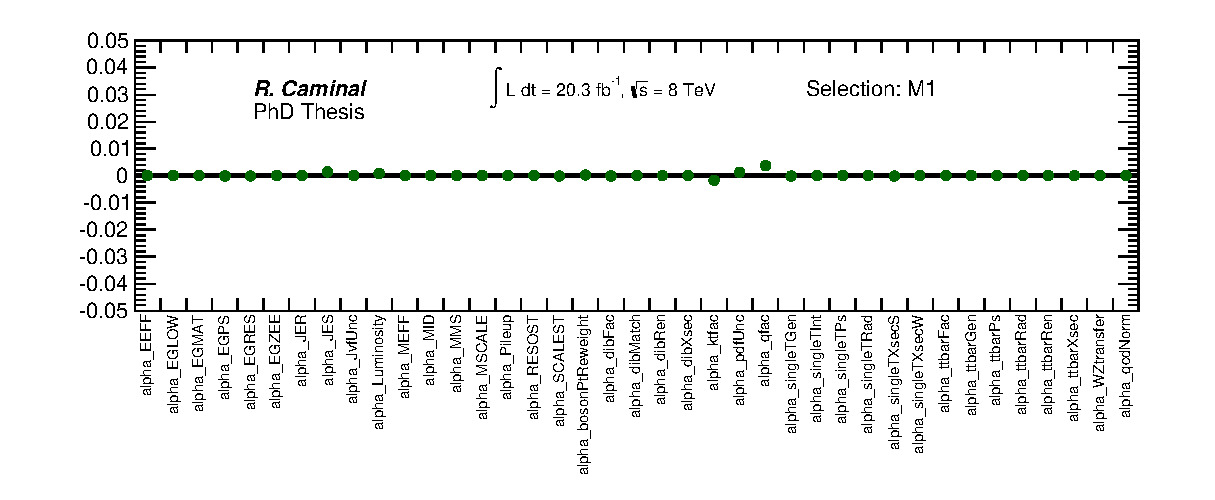
\includegraphics[width=0.995\textwidth]{MonojetAnalysis/Figures/NuisanceParamsZoomPlot_Stop_M1.eps}
    }
    \mbox{
      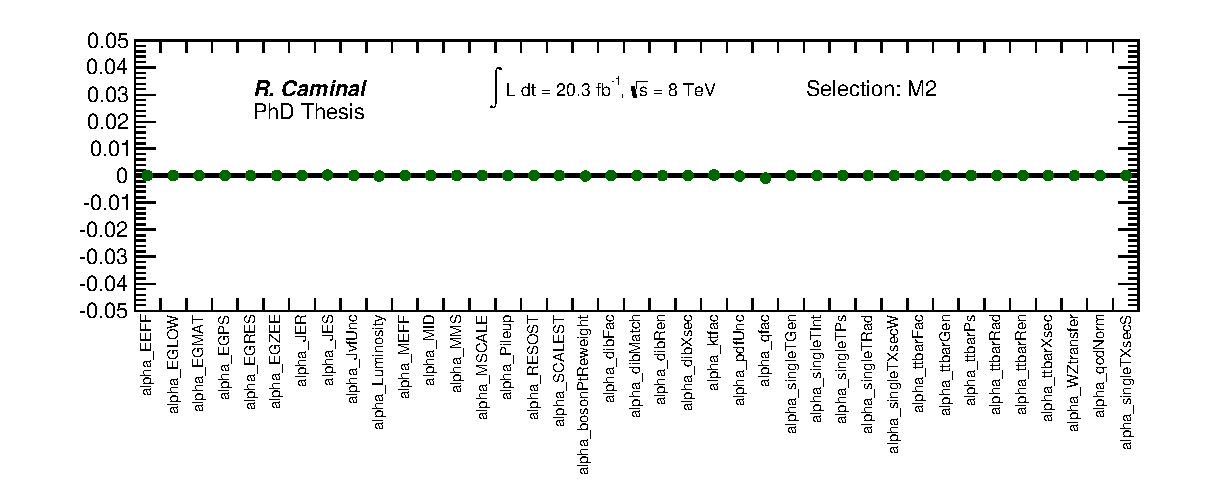
\includegraphics[width=0.995\textwidth]{MonojetAnalysis/Figures/NuisanceParamsZoomPlot_Stop_M2.eps}
    }
    \mbox{
      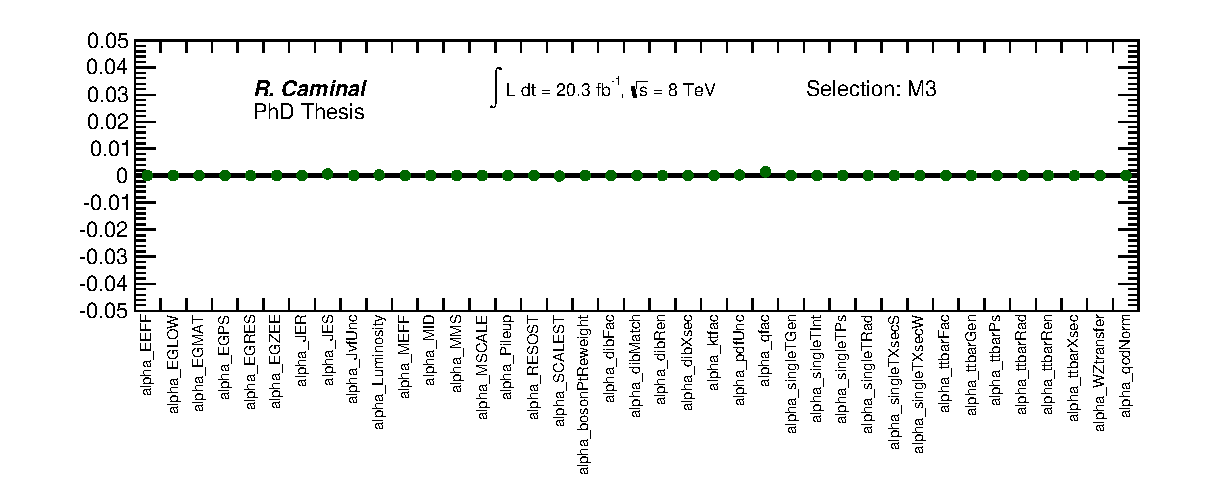
\includegraphics[width=0.995\textwidth]{MonojetAnalysis/Figures/NuisanceParamsZoomPlot_Stop_M3.eps}
    }
  \end{center}
  \caption[Nuisance parameter values after the global fits with the background-only setup in the M1 to M3 signal selections.]{Values for the nuisance parameters after the global fits with the background-only setup in the M1 to M3 signal selections. The points do not include uncertainties.}
  \label{fig:corrMatrix_M1M2M3}
\end{figure}

\begin{figure}[!ht]
  \begin{center}
    \mbox{
      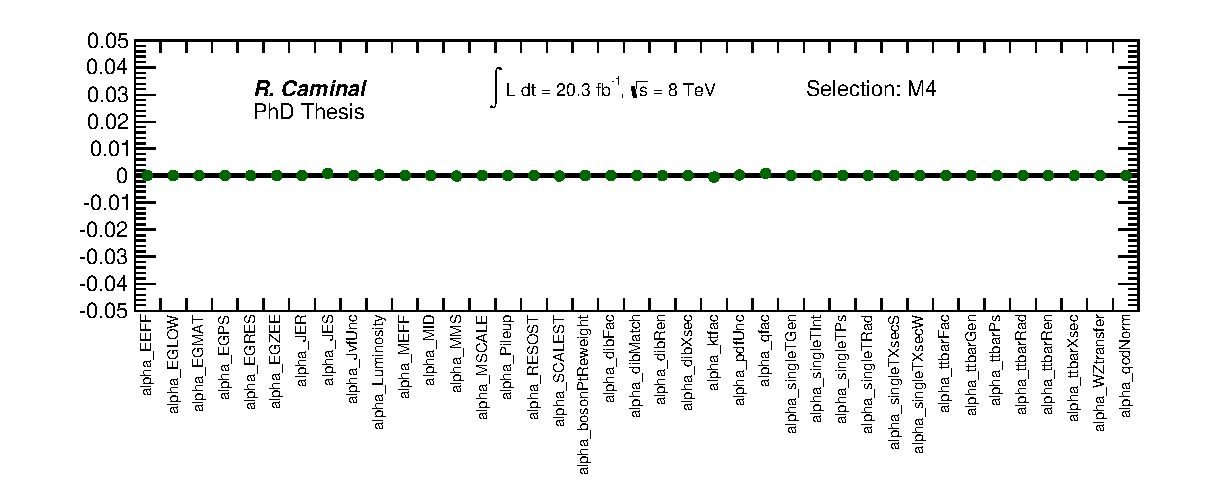
\includegraphics[width=0.995\textwidth]{MonojetAnalysis/Figures/NuisanceParamsZoomPlot_Stop_M4.eps}
    }
    \mbox{
      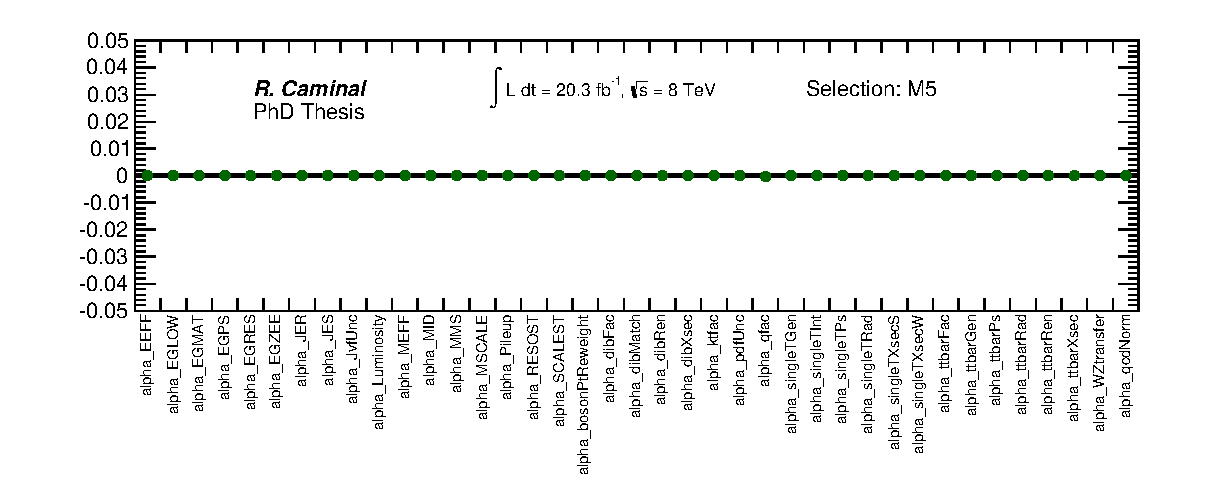
\includegraphics[width=0.995\textwidth]{MonojetAnalysis/Figures/NuisanceParamsZoomPlot_Stop_M5.eps}
    }
    \mbox{
      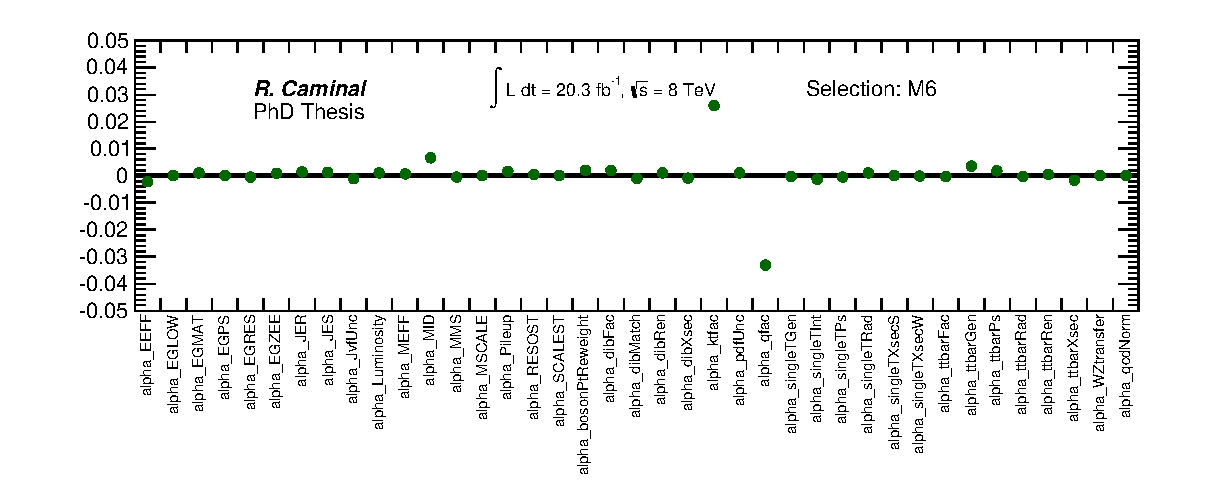
\includegraphics[width=0.995\textwidth]{MonojetAnalysis/Figures/NuisanceParamsZoomPlot_Stop_M6.eps}
    }
  \end{center}
  \caption[Nuisance parameter values after the global fits with the background-only setup in the M4 to M6 signal selections.]{Values for the nuisance parameters after the global fits with the background-only setup in the M4 to M6 signal selections. The points do not include uncertainties}
  \label{fig:corrMatrix_M4M5M6}
\end{figure}
